% Chapter Template

\chapter{Chapter 1: Introduction} % Main chapter title

\label{Chapter1} % Change X to a consecutive number; for referencing this chapter elsewhere, use \ref{ChapterX}

%----------------------------------------------------------------------------------------
%	SECTION 1
%----------------------------------------------------------------------------------------

\section{Historical Context}
%-----------------------------------
%	SUBSECTION 1
%-----------------------------------
\subsection{Hierarchy Models}
\par Hubel and Wiesel (1962) classified primary visual cortex (V1) neurons into simple cells and complex cells. The essential difference between the simple cells and complex cells is that the responses of simple cells are modulated by the spatial phase of a sine grating, whereas the responses of complex cells are largely phase invariant. In other words, as we progress from simple cells to complex cells, the neurons become selective for increasingly complex stimuli and at the same time become more tolerant to the exact position within their receptive fields. 

\par Based on this, a natural way to construct complex cells is to group responses from simple cells with the same orientation preference, but with different phase preferences.

\par This idea directly inspired the Neocognitron model:  S-cells are tuned to simple stimuli after a few operations (convolution) and then they are combined (by pooling through maximum or average) to form C-cells tuned to more complex stimuli. 

\par The Neocognitron model is among a myriad of hierarchical models of the visual system. They differ in their specific wiring, parameterizations, and the mathematical operations. But all of these models has a common basic structure, Hmax:
\begin{figure}[H]
\centering
    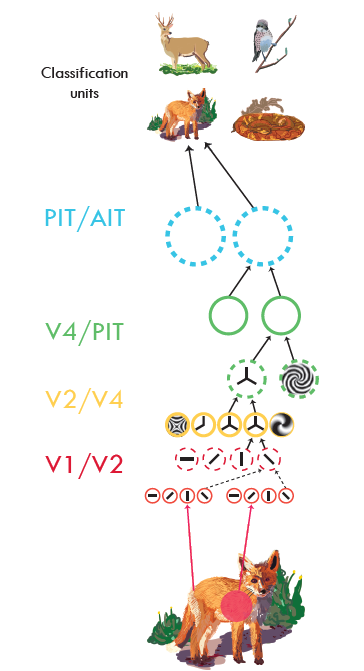
\includegraphics[width=7cm]{figures/models/hmax.png}
     \caption{An Intuitive Illustration of Hmax (Serre, 2014)}
\end{figure}

The figure below shows a systematic illustration of the general idea behind the hierarchical models:
\begin{figure}[H]
\centering
    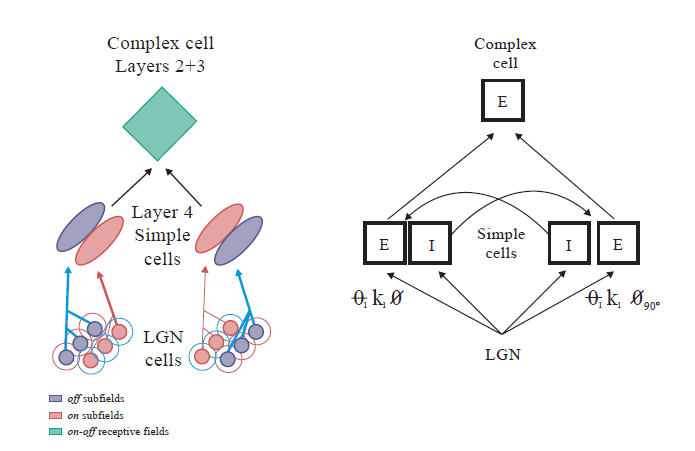
\includegraphics[width=10cm]{figures/models/hierarchical-models.png}
     \caption{Illustration of the hierarchical models (Martinez and Alonso, 2003)}
\end{figure}

The possible advantages of hierarchical models are as follows:
\begin{itemize}
    \item If a visual recognition task can be decomposed into low-complexity learning tasks for each layer of a hierarchical learning machine, then each layer may require only a small number of training examples (Poggio and Smale, 2003).
    \item The lowest levels of the hierarchy may represent a dictionary of features that can be shared across multiple classification tasks (Geman, 1999), thus increasing efficiency.
\end{itemize}

There are also some known limitations of hierarchical models:
\begin{itemize}
    \item Hierarchical models assume that the computations at each successive stage being largely feedforward (Riesenhuber and Poggio, 1999; DiCarlo et al., 2012). This is limited because back-projections are also likely to be a key part of the visual system. 
    \item There remains a very broad distribution of tuning and receptive field sizes in all areas of the visual hierarchy. Hence, the anatomical hierarchy should be taken as an idealization and cannot be taken as a strict flowchart of visual information (Hegde and Felleman, 2007). 
    \par One particularly interesting piece of evidence: A close comparison of shape representation between V1, V2 and V4 also demonstrated a complex pattern of shape selectivity with significant deviation from strict hierarchical organization with some cells in V1 exhibiting more complex tuning than some cells in V4 (Hegde and Van Essen, 2007).
\end{itemize}


%-----------------------------------
%	SUBSECTION 2
%-----------------------------------

\subsection{Alternative Models}
Since Hubel and Wiesel (1962) proposed the classification of simple cells and complex cells, many other hierarchical models have been proposed for a more realistic representation for the cortical circuitry. Furthermore, new experimental and computational evidence provided serious alternatives to this hierarchical model, including parallel models and recurrent models (Martinez and Alonso, 2003). There are still many controversies and debates over which models best capture mechanisms of the visual system.

\subsubsection{Parallel Models}
The first strong evidence against the hierarchical model was the discovery that some complex cells, like simple cells, receive monosynaptic input from the thalamus (Hoffmann and Stone 1971). Based on this discovery, Hoffman and Stone proposed that both cell types, simple and complex, were generated in parallel by separate thalamocortical pathways (Hoffman and Stone 1971), as shown in diagram A in Figure 4. 
\begin{figure}[H]
\centering
    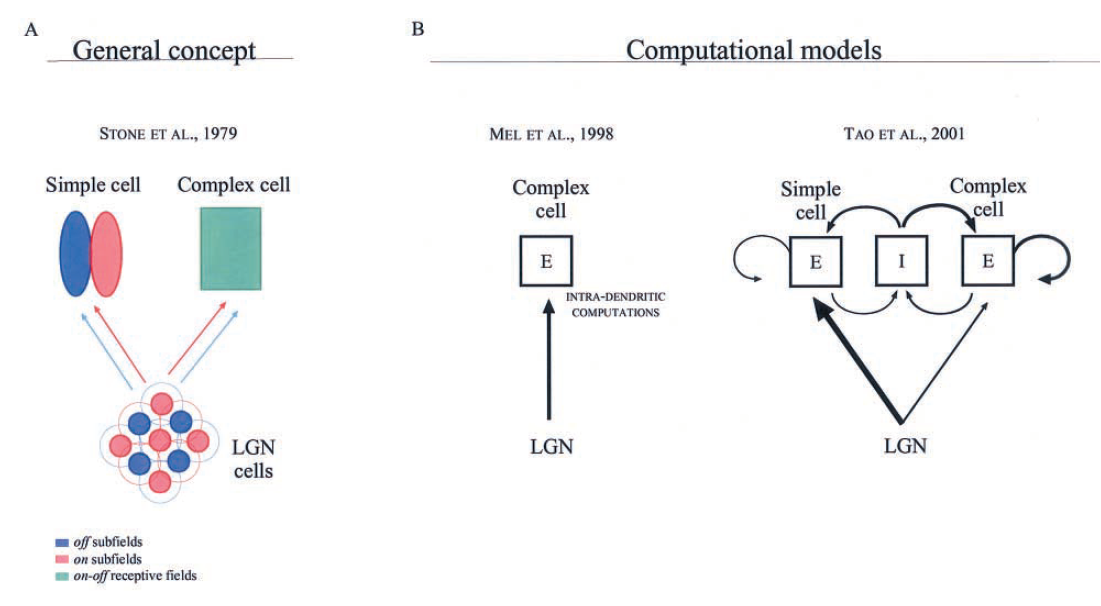
\includegraphics[width=10cm]{figures/models/parallel-models.png}
     \caption{Illustration of the parallel models (Martinez and Alonso, 2003)}
\end{figure}

Simple cells and complex cells are far from being two parallel cortical pathways in the same way that X and Y cells are parallel thalamic pathways. However, the idea that some complex receptive fields can be generated at
least in part by direct thalamic inputs is likely to be correct. (Martinez and Alonso, 2003)

\subsubsection{Recurrent Models}
Recurrent models changed the focus of attention from single cells to networks of cortical connections. (Martinez and Alonso, 2003) An illustration for recurrent models are shown in Figure 5.

\begin{figure}[H]
\centering
    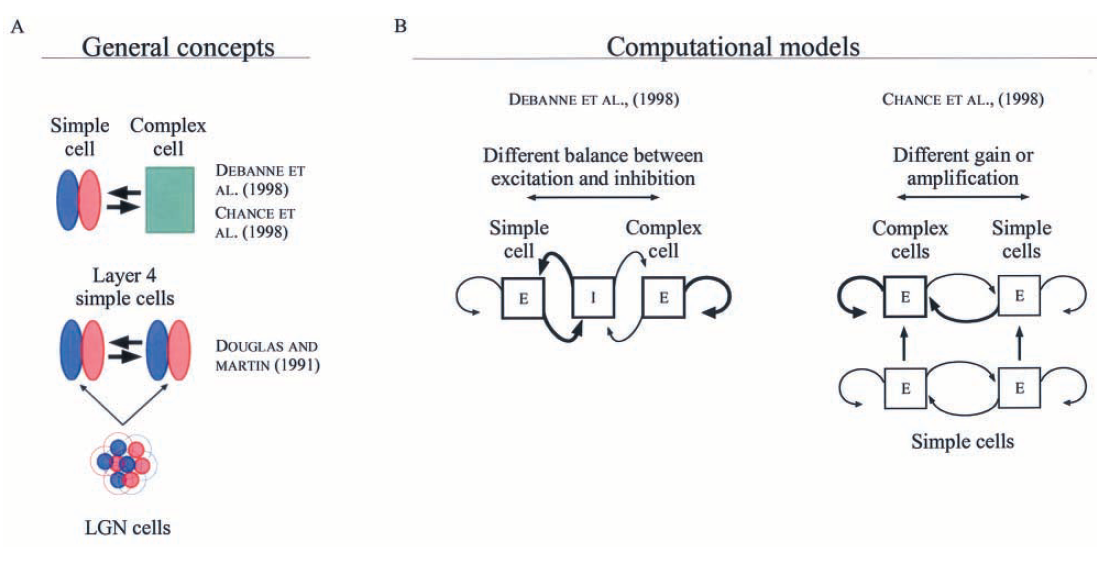
\includegraphics[width=10cm]{figures/models/recurrent-models.png}
     \caption{Illustration of the recurrent models (Martinez and Alonso, 2003)}
\end{figure}

%----------------------------------------------------------------------------------------
%	SECTION 2
%----------------------------------------------------------------------------------------

\section{Literature Review}


\section{Goals and Significance}